\documentclass{beamer}
\usepackage[latin1]{inputenc}
\usetheme{Boadilla}
\title[Integrated Lecture Management]{A proposal for the practical assignment in MoC 2011}
\date{\today}
\institute{IAM}
\author{Cedric Reginster, Bjoern Mosler}

\begin{document}

\begin{frame}
	\titlepage
\end{frame}


\begin{frame}{Overview}
	\tableofcontents
\end{frame}

\begin{frame}{Basic Idea}

	\section{Basic Idea}
	Facilitate lecture management by integrating EVUBS, Google Calendar and Google Maps.

\end{frame}

\begin{frame}{EVUBS}

	\section{Services}
	\subsection{EVUBS}

	\begin{columns}
		\begin{column}{0.5\textwidth}
			\begin{itemize}
				\item A web service which provides lecture data for Uni Bern.
				\item allows us to mimic \url{www.evub.unibe.ch}.
			\end{itemize}
		\end{column}

		\begin{column}{0.5\textwidth}
			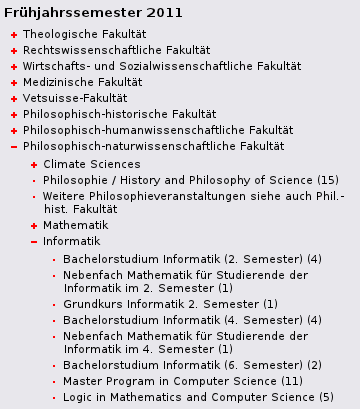
\includegraphics[scale=0.5]{evub.png} 
		\end{column}
	\end{columns}

\end{frame}

\begin{frame}{Google Calendar \& Google Maps}
	\subsection{Google Calendar \& Maps}
	Who does not know them?
\end{frame}

\begin{frame}{Application details}
	\section{Application details}

	\begin{itemize}
		\item Allow users to browse lectures like in EVUB.
		\item Allow user to ``subscribe'' to a lecture.
		\item Show subscriptions on home screen for convenient access.
	\end{itemize}

	After subscription:
	\begin{itemize}
		\item Present route from current location to location where lecture takes place using Google Maps.
		\item Automatically add lecture as an appointment to Google Calendar.
		\item User may create tasks belonging to a lecture, would also be added to Google Calendar.
	\end{itemize}
	
\end{frame}

\begin{frame}{Home screen prototype}
	\subsection{Home screen prototype}
	
	\begin{center}
		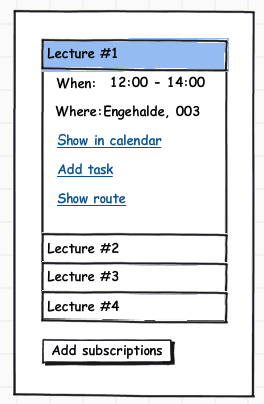
\includegraphics[scale=0.5]{home.png}
	\end{center}

\end{frame}

\begin{frame}{Further features}

	\section{Further features}
	
	\begin{itemize}
		\item Generate printable timetable from subscriptions.
		\item Add reminders based on subscriptions.
	\end{itemize}
\end{frame}
	
\end{document}